\chapter{Tutorial}\label{tutorial}

\section{Basic System Dynamics model}

In 1965, Richard Goodwin, the great pioneer of complexity in
economics, presented the paper \htmladdnormallink{``A Growth
Cycle''}{https://en.wikipedia.org/wiki/Goodwin_model_(economics)} to
the First World Congress of the Econometric Society in Rome. It was
later published in a book collection (Goodwin, Richard M. 1967. "A
Growth Cycle," in C. H. Feinstein, {\em Socialism, Capitalism and Economic
Growth}. Cambridge: Cambridge University Press, pp. 54--58.); to my
knowledge it was never published in a journal. 

Goodwin's model has been subjected to much critical literature about
implying stable cycles, not matching empirical data, etc., but Goodwin
himself emphasized that it was a ``starkly schematized and hence quite
unrealistic model of cycles in growth rates". He argued however that
it was a better foundation for a more realistic model than ``the more
usual treatment of growth theory or of cycle theory, separately or in
combination.'' 

Goodwin emphasized the similarity of this model to the Lokta-Volterra
model of interacting predator and prey, which can make it seem as if
it was derived by analogy to the biological model. But in fact it can
easily be derived from a highly simplified causal chain:

\begin{itemize}

\item The level of output ($Y$) determines the level of employment ($L$), with $L=Y/a$ where $a$ is a measure of labor productivity;
\item Given a population $N$, the employment rate $\lambda=L/N$ plays
a role in determining the {\bf\em rate of change} of the wage $w$:
Goodwin used a linear approximation to a non-linear ``Phillips
Curve'': 

%\fwhtmladdimg{NewItem55.png}
\begin{center}
  \includegraphics{images/PhillipsCurve.eps}
\end{center}

His linear approximation was:

\begin{displaymath}
\frac1w\frac{d}{dt}w=-\gamma+\rho\cdot\lambda
\end{displaymath}

\item In a simple two-class model, profits $\Pi$ equals the level of
output $Y$ minus the wage bill: $\Pi=Y-wL$ 
\item For simplicity, Goodwin assumed that all profits were invested, so that Investment equals profits: $I=\Pi$.
\item Investment is the rate of change of the capital stock $K$;
\item The level of output is, to a first approximation, determined by
the level of capital stock ($K$). A simple way of stating this is that
$Y$ is proportional to $K$: $Y=K/v$, where $v$ is a constant (Goodwin
notes that this relation ``could be softened but it would mean a
serious complicating of the structure of the model''); and finally 
\item Goodwin assumed that labor productivity grew at a constant rate $\alpha$, while population grew at a constant rate $\beta$.

Goodwin published the model as a reduced form equation in the two
system states the employment rate ($\lambda$) and the workers' share
of output ($\omega$): 

\begin{eqnarray*}
\frac{d}{dt}\lambda&=&\lambda\left(\frac{1-\omega}{v}-\alpha-\beta\right)\\
\frac{d}{dt}\omega&=&\omega\cdot\left(\rho\cdot\lambda-\gamma-\alpha\right)
\end{eqnarray*}

\end{itemize}

This form is useful for analytic reasons, but it obscures the causal
chain that actually lies behind the model. With modern system dynamic
software, this can be laid out explicitly, and we can also use much
more meaningful names. We'll start with defining output (which is a
variable). Click on \buttonIcon{var.eps} on the Icon Palette, or
click on the Operations menu and choose ``Variable''. This will open
up the ``Specify Variable Name'' window:

\begin{center}
\scalebox{0.5}{\htmladdimg{NewItem63.png}}
\end{center}

Enter ``{\em\bf GDP}'' into the ``Name'' field, and leave the other
fields blank---since {\em\bf GDP} is a variable and we're defining a
dynamic system, the value of {\em\bf GDP} at any particular point in
time will depend on the other entities in the model. Now Click OK (or
press ``Enter''). The variable will now appear, attached to the
cursor. Move to a point near the top of the screen and click, which
will place the variable at that location.

We are now going to write the first part of the model, that Labor
({\em\bf Labor}) equals output ({\em\bf GDP}) divided by labor
productivity ({\em\bf LabProd}). Just for the sake of illustration,
we'll make {\em\bf a} a parameter, which is a named constant (this can
easily be modified later). For this we start by clicking on
\buttonIcon{const.eps} on the Palette, or by choosing
Insert/variable from the menu. This will pop-up the Edit Constant
window:

\begin{center}
\scalebox{0.5}{\htmladdimg{NewItem66.png}} 
\end{center}

There is actually no real difference between the ``Edit constant''
dialog and the ``Edit variable'' dialog. The window's title differs,
and the default value of Type is ``constant'' instead of
``flow''. We're going to select ``parameter'', allowing one to give
the parameter a name.

Give the paramter the name ``{\em\bf LabProd}'' and the value of 1
(i.e., one unit of output per worker). Click OK or press Enter and the
constant \buttonIcon{LabProd.eps}  will now be attached to the
cursor. Place it below {\em\bf GDP}: 

\begin{center}
\scalebox{0.5}{\htmladdimg{NewItem66.png}}
\end{center}

Now we need to divide {\em\bf GDP} by {\em\bf LabProd}. Click on the
\buttonIcon{divide.eps} symbol on the palette and the symbol will
be attached to the cursor. Drag it near the other two objects and
click. Your Canvas will now look something like this: 

\begin{center}
\includegraphics{images/NewItem70.eps} 
\end{center}

Now to complete the equation, you have to attach {\em\bf GDP}  to the top of the
divide block and LabProd to the bottom.

Now move your cursor to the right hand side of
\buttonIcon{GDP.eps}  and click, hold the mouse button down, and
drag. An arrow will come out from  \buttonIcon{GDP.eps}. Drag
this arrow to the top of the divide block (where you'll see a tiny
multiply sign) and release the mouse. You should then see this: 

\begin{center}
\includegraphics{images/NewItem74.eps} 
\end{center}


When the mouse hovers over a block, you will then see little
circles that identify the input and output ports of the block: 

\begin{center}
\includegraphics{images/NewItem75.eps} 
\end{center}

Those are the connection points for wires, so start dragging from one
and release on the other. Now wire LabProd to the bottom of the Divide
block (where you'll see a miniature divide symbol (blown up below): 

\begin{center}
\includegraphics{images/NewItem76.eps} 
\end{center}

Then click on \buttonIcon{var.eps} in the Design Icons to create a new variable, call it
Labor, place it the the right of the Divide block, and wire the output port from the Divide block to the
input port for {\bf\em Labor}: 

\begin{center}
\includegraphics{images/NewItem79.eps} 
\end{center}


To show the correspondence between the flowchart above and standard
modeling equations, click on the equations tab: 

\begin{eqnarray*}
\mathrm{GDP}&=&\\
\mathrm{Labor}&=&\frac{\mathrm{GDP}}{\mathrm{LabProd}}\\
\end{eqnarray*}

Now let's keep going with the model. With {\bf\em Labor} defined, the
employment rate will be {\bf\em  Labor} divided by {\bf\em
Population}. Define {\bf\em Population} as a parameter (we'll later
change it to a variable), and give it a value of 110. 

\begin{center}
\scalebox{0.5}{\htmladdimg{NewItem81.png}}
\end{center}

Add it to the Canvas and you are now ready to define the employment
rate---another variable. Click on \buttonIcon{var.eps}, give it
the name ``$\backslash$lambda'' (be sure to include the backslash symbol), put
another Divide block on the canvas, choose Wire mode and wire this
next part of the model up. You should now have:

\begin{center}
\includegraphics{images/NewItem83.eps}
\end{center}


Now switch to the equations tab, and you will see

\begin{eqnarray*}
\mathrm{GDP}&=&\\
\mathrm{Labor}&=&\frac{\mathrm{GDP}}{\mathrm{LabProd}}\\
\lambda&=&\frac{\mathrm{Labor}}{\mathrm{Population}}\\
\end{eqnarray*}

Notice that Minsky outputs a Greek $\lambda$ in the equation. You can
input such characters directly, if your keyboard supports them as unicode
characters, however you can also use a subset of the LaTeX language to give
your variables more mathematial names.


With the employment rate defined, we are now ready to define a
``Phillips Curve'' relationship between the level of employment and the
{\em\bf rate of change} of wages. There was far more to Phillips than this (he
actually tried to introduce economists to system dynamics back in the
1950s), and far more to his employment-wage change relation too, and
he insisted that the relationship was nonlinear (as in Goodwin's
figure above). But again for simplicity we'll define a linear
relationship between employment and the rate of change of wages. 

Here we need to manipulate the basic linear equation that Goodwin used:

\begin{displaymath}
\frac1w\frac d{dt}w = -\gamma+\rho\cdot\lambda
\end{displaymath}

Firstly multiply both sides by $w$:

\begin{displaymath}
\frac d{dt}w = w\cdot(-\gamma+\rho\cdot\lambda)
\end{displaymath}

Then integrate both sides (because integration is a numerically much
more stable process than differentiation, all system dynamics programs
use integration rather than differentiation): 

\begin{displaymath}
w=w_0+\int w\cdot(-\gamma+\rho\cdot\lambda)
\end{displaymath}

In English, this says that the wage now is the initial wage plus the
integral of the wage multiplied by its rate of change function. That's
what we now need to add to the Canvas, and the first step is to spell
out the wage change function itself. Firstly, since we're using a
linear wage response function, the rate of employment has to be
referenced to a rate of employment at which the rate of changes is
zero.  I suggest using Milton Friedman's concept of a
``Non-Accelerating-Inflation-Rate-of-Unemployment'', or NAIRU. We need
to define this constant, subtract it from 1, and subtract the result
from the actual employment rate $\lambda$. To enter 1, click on
\buttonIcon{const.eps}, define a constant and give it
a value of 1. Then define another variable NAIRU, and give it a value
of 0.05 (5\% unemployment). Select ``parameter'' as the variable
type. Subtract this from 1 and subtract the result from $\lambda$. You
should have the following:

\begin{center}
  \includegraphics{images/NewItem108.eps}
\end{center}

Now we need to multiply this gap between the actual employment rate
and the ``NAIRE'' rate by a parameter that represents the response of
wages to this gap. Let's call this parameter {\bf\em Emp\_\{Response\}} (remember to include the underscore and the braces). Define the parameter, give it a value of 10, and multiply ($\lambda$ minus NAIRE) by it:

\begin{center}
\resizebox{\textwidth}{!}{\includegraphics{images/NewItem109.eps}}
\end{center}

Now we are ready to add a crucial component of a dynamic model: the
integral block, which takes a flow as its input and has the integral
of that flow as the output. The wage rate {\bf\em w} is such a variable, and we
define it by clicking on the \buttonIcon{int.eps} symbol in the Icon Palette (or by
choosing Operations/Integrate from the {\em Insert} menu). This then attaches the
following block to the cursor: 

\begin{center}

\includegraphics{images/NewItem39.eps}
\end{center}


Now we need to rename this from the default name of ``int1'' to
``{\em\bf w}'' for the wage rate. Either right click or double-click
on ``int1'' and this will bring up the edit window . Rename it to ``w'' and
give it a value of 1: 

\begin{center}
\scalebox{0.5}{\htmladdimg{NewItem93.png}}
\end{center}

To compete the integral equation, we need to multiply the linear
employment response function by the current wage before we integrate
it (see the last equation above). There are two ways to do
this. First, place a multiply block between the wage change function
and the integral block, wire the function up to one input on the
multiply block, and then either:

\begin{itemize}
\item wire the output of the {\bf\em w} block back to the other input
on multiply block; or
\item Right-click on {\bf\em w}, choose ``Copy Var'', place that copy
before the multiply block, and wire it up.
\end{itemize}

The first method gives you this initial result:

\begin{center}
\includegraphics{images/NewItem110.eps}
\end{center}

That looks messy, but notice the blue dot on the wire? Click and drag
on that and you will turn the straight line connector into a curve: 

\begin{center}
\resizebox{\textwidth}{!}{\includegraphics{images/NewItem111.eps}}
\end{center}

The second approach, which I personally prefer (it's neater, and it
precisely emulates the integral equation), yields this result: 

\begin{center}
\resizebox{\textwidth}{!}{\includegraphics{images/NewItem112.eps}}
\end{center}

From this point on the model develops easily---``like money for old
rope'', as one of my maths lecturers used to say. Firstly if we
multiply the wage rate {\bf\em w} by {\bf\em Labor} we get the {\em\bf
Wage Bill}. To do this,
firstly create the variable Wage Bill, and put it well below where $w$
currently is on your diagram: 

\begin{center}
\resizebox{\textwidth}{!}{\includegraphics{images/NewItem113.eps}}
\end{center}

Now right-click on {\bf\em WageBill} and choose ``Flip''. This rotates
the block through 180 degrees (any arbitrary rotation can be applied
from the variable definition window itself). Now right-click on
{\bf\em Labor}, which you've already defined some time ago, and choose
``Copy''. Place the copy of {\bf\em Labor} to the right of {\bf\em
WageBill}:

\begin{center}

\includegraphics{images/NewItem98.eps}
\end{center}

Now insert a multiply block before {\bf\em WageBill}, and wire {\bf\em
w} and {\bf\em Labor} up to it. Curve the wire from $w$ using the blue
dots (you can do this multiple times to create a very curved path:
each time you create a curve, another 2 curve points are added that
you can also manipulate, as I have done below: 

\begin{center}
\resizebox{\textwidth}{!}{\includegraphics{images/NewItem114.eps}}
\end{center}


The next step is to subtract the {\bf\em WageBill} from {\bf\em GDP}
to define {\bf\em Profits}. Take a copy of {\bf\em GDP}, insert it
above {\bf\em WageBill}, insert a subtract block, and wire it up to
define the variable {\bf\em Profits}:

\begin{center}
\includegraphics{images/NewItem100.eps}
\end{center}


In the simple Goodwin model, all Profits are invested, and investment
of course is the rate of change of the capital stock Capital. Create a
variable called Investment, wire this up to Profits, and then create a
new integral variable {\em Capital} using the \buttonIcon{int.eps}
icon. Right-click or double-click on it to rename {\em int2} to {\em
Capital}, and give it an initial value of 300:

\begin{center}
\scalebox{0.5}{\htmladdimg{NewItem102.png}}
\end{center}

Wire this up to Investment:

\begin{center}
\includegraphics{images/NewItem104.eps}
\end{center}

Now there's only one step left to complete the model: define a
parameter CapOutputRatio and give it a value of 3:

\begin{center}
\scalebox{0.5}{\htmladdimg{NewItem103.png}}
\end{center}


Divide Capital by this, and wire the result up to the input on
GDP. You have now built your first dynamic model in Minsky: 


Before you attempt to run it, do two things. Firstly from the {\em Runge
Kutta} menu item, change the Max Step Size to 0.01---to get a smoother
simulation. 

\begin{center}
\scalebox{0.5}{\htmladdimg{NewItem107.png}}
\end{center}

Secondly, add some graphs by clicking on the
\smhtmladdimg{plot.png} icon, placing the graph
in the middle of the flowchart, and wiring up $\lambda$ and $w$ to two of
the four inputs on the left hand side. You will now see that, rather
than reaching equilibrium, the model cycles constantly:

\begin{center}
\resizebox{\textwidth}{!}{\includegraphics{images/NewItem116.eps}}
\end{center}

If you click on the equations tab, you will see that you have defined the following system of
equations:

\begin{eqnarray*}
\mathrm{GDP}&=&\frac{\mathrm{Capital}}{\mathrm{CapOutRatio}}\\
\mathrm{Investment}&=&\mathrm{Profits}\\
\mathrm{Labor}&=&\frac{\mathrm{GDP}}{\mathrm{LabProd}}\\
\mathrm{Profits}&=&\mathrm{GDP}-\mathrm{WageBill}\\
\mathrm{WageBill}&=&w\times\mathrm{Labor}\\
\lambda&=&\frac{\mathrm{Labor}}{\mathrm{Population}}\\
\omega&=&\frac{\mathrm{WageBill}}{\mathrm{GDP}}\\
\frac{dw}{dt}&=&\mathrm{Emp}_\mathrm{Response}\times(\lambda-(1-\mathrm{NAIRU})
        \times w\\
\frac{d\mathrm{Capital}}{dt}&=&\mathrm{Investment}\\
\end{eqnarray*}


At this level of complexity, the equation form---if you're accustomed
to working in equations---is as accessible as the block diagram model from
which it was generated. But at much higher levels of complexity, the
block diagram is far easier to understand since it displays the causal
links in the model clearly, and can be structured in sub-groups that
focus on particular parts of the system. 

\section{Basic Banking model}\label{tut:basicBankModel}

If you haven't yet read the section on \htmlref{Creating a Banking
Model}{creatingBankingModel}, do so now. This tutorial starts from the
skeleton of the ``Loanable Funds'' model built in that section, and
using \htmlref{time constants}{time-constants} to specify how quickly
lending occurs.  


\subsection{Loanable Funds}

Our model begins with the single operation of Patient lending to
Impatient at a rate that, if kept constant at its initial level of of
\$10 per annum, would empty the Patient account in 10 years. Because
the rate of outflow declines as the Patient account declines, the
money in the account decays towards zero but never quite reaches it.

%\begin{center}
%\begin{tabular}{|c|cccc|}
%\hline
%Flows $\downarrow$ / Stock Variables $\rightarrow$&\multicolumn{1}{|c|}{$Reserves$}&\multicolumn{1}{|c|}{$Patient$}&\multicolumn{1}{|c|}{$Impatient$}&\multicolumn{1}{|c|}{$Safe$}\\\cline{2-5}&\multicolumn{1}{|c|}{asset}&\multicolumn{2}{|c|}{liability}&\multicolumn{1}{|c|}{equity}\\\hline
%Initial Conditions&$120$&$100$&$0$&$20$\\
%Patient lends to Impatient&&$-Lend$&$Lend$&\\
%\hline
%\end{tabular}
%\resizebox{\textwidth}{!}{\includegraphics{images/NewItem169.eps}}
%\end{center}
\begin{center}
  \scalebox{.5}{\includegraphics{images/godleyTableWithAccounts5.eps}}
\end{center}

Many more actions need to be added to this model to complete it. For a
start, Impatient should be paying interest to Patient on the amount
lent. Add an additional row to the Godley Table by clicking on the
`+' key
next to ``Patient lends to Impatient'' to create a blank row:

%\begin{center}
%\begin{tabular}{|c|cccc|}
%\hline
%Flows $\downarrow$ / Stock Variables $\rightarrow$&\multicolumn{1}{|c|}{$Reserves$}&\multicolumn{1}{|c|}{$Patient$}&\multicolumn{1}{|c|}{$Impatient$}&\multicolumn{1}{|c|}{$Safe$}\\\cline{2-5}&\multicolumn{1}{|c|}{asset}&\multicolumn{2}{|c|}{liability}&\multicolumn{1}{|c|}{equity}\\\hline
%Initial Conditions&$120$&$100$&$0$&$20$\\
%Patient lends to Impatient&&$-Lend$&$Lend$&\\
%&&&&\\
%\hline
%\end{tabular}
%\end{center}
\begin{center}
  \scalebox{.5}{\includegraphics{images/godleyTableWithAccounts6.eps}}
\end{center}

Then label this flow ``Impatient pays interest'' and make the entry
``Interest'' into the cell for Patient on that row. Make the matching
entry ``-Interest'' in the cell for Impatient. The flow ``Interest'' now
appears on the input side of the Godley Table on the Canvas: 

%\begin{center}
%\begin{tabular}{|c|cccc|}
%\hline
%Flows $\downarrow$ / Stock Variables $\rightarrow$&\multicolumn{1}{|c|}{$Reserves$}&\multicolumn{1}{|c|}{$Patient$}&\multicolumn{1}{|c|}{$Impatient$}&\multicolumn{1}{|c|}{$Safe$}\\\cline{2-5}&\multicolumn{1}{|c|}{asset}&\multicolumn{2}{|c|}{liability}&\multicolumn{1}{|c|}{equity}\\\hline
%Initial Conditions&$120$&$100$&$0$&$20$\\
%Patient lends to Impatient&&$-Lend$&$Lend$&\\
%Impatient pays interest&&$Interest$&$-Interest$&\\
%\hline
%\end{tabular}
%\end{center}
\begin{center}
  \scalebox{.5}{\includegraphics{images/godleyTableWithAccounts7.eps}}
\end{center}

Interest now has to be defined. It will be the amount in Impatient's
account (since this began at zero) multiplied by the rate of interest
charged by Patient:

\begin{center}
\includegraphics{images/NewItem173.eps}
\end{center}

With that definition, the dynamics of the model change: rather than
the Patient account falling to zero and Impatient rising to 100, the
two accounts stabilize once the outflow of new loans by Patient equals
the inflow of interest payments by Impatient:

\begin{center}
\resizebox{\textwidth}{!}{\includegraphics{images/NewItem174.eps}}
\end{center}

Though it stabilizes, this is is still a very incomplete model:
neither Patient nor Impatient are doing anything with the money apart
from lending it and paying interest. I am now going to assume that
Impatient is borrowing the money in order to hire workers to work at a
factory and produce output for sale. So we now need another account
called Workers, and a payment from Impatient to Workers called Wage:

%{
%  \noindent
%\small
%\begin{tabular}{|c|ccccc|}
%\hline
%Flows $\downarrow$ / Stock Variables $\rightarrow$&\multicolumn{1}{|c|}{$Reserves$}&\multicolumn{1}{|c|}{$Patient$}&\multicolumn{1}{|c|}{$Impatient$}&\multicolumn{1}{|c|}{$Workers$}&\multicolumn{1}{|c|}{$Safe$}\\\cline{2-6}&\multicolumn{1}{|c|}{asset}&\multicolumn{3}{|c|}{liability}&\multicolumn{1}{|c|}{equity}\\\hline
%Initial Conditions&$120$&$100$&$0$&$0$&$20$\\
%Patient lends to Impatient&&$-Lend$&$Lend$&&\\
%Impatient pays interest&&$Interest$&$-Interest$&&\\
%Impatient pays Workers&&&$-Wage$&$Wage$&\\
%\hline
%\end{tabular}
%}
\begin{center}
  \scalebox{.5}{\includegraphics{images/godleyTableWithAccounts8.eps}}
\end{center}

In a more complex model, the Wage bill could be related to the current
rate times the number of workers in employment. In this simple model I
will regard the wage as a function of the amount of money in
Impatient's account turning over several times a year in the payment
of wages. Using a time constant, I will assume that the amount in
Impatient's account turns over 3 times a year paying wages, so that
the time constant $\tau_T$ is 1/3rd of a year:

\begin{center}
  \includegraphics{images/NewItem176.eps}
\end{center}

The dynamics of this incomplete model are very different again: very
little money turns up in the Impatient account, and all of the money
ends up in the Workers account. However economic activity also ceases
as both lending and the flow of wages falls towards zero:

\begin{center}
  \resizebox{\textwidth}{!}{\includegraphics{images/NewItem177.eps}}
\end{center}

This is because wages are being paid to workers, but they are doing
nothing with it. So we need to include consumption by workers--and by
Patient as well. Here the reason time constants are useful may be more
obvious. The time constant for consumption by Workers is given the
very low value of 0.05---or 1/20th of a year---which indicates that if
their initial rate of consumption was maintained without any wage
income, they would reduce their bank balances to zero in 1/20th of a
year or about 2.5 weeks.
